\documentclass[tikz,convert={outfile=\jobname.svg}]{standalone}\usepackage{pgfplots}

\pgfplotsset{
	compat = 1.5.1,
	axis equal
	%width = 1.2\linewidth,
	%height = 1.2\linewidth
}

\begin{document}

%\begin{figure}[t]
%  \centering
  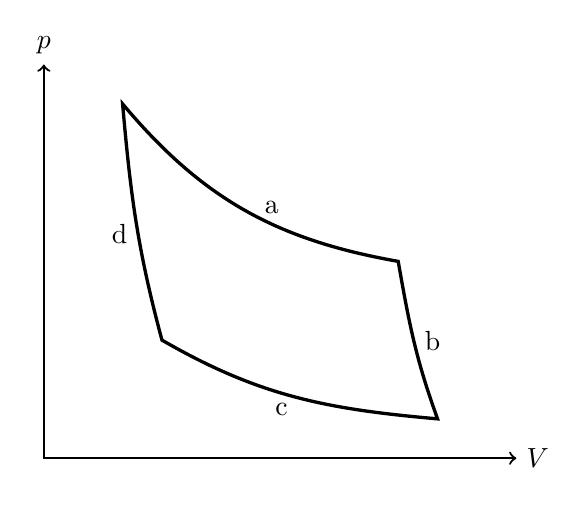
\begin{tikzpicture}[thick]
    \draw[<->]
      (0,5) node[above]{$p$} -- (0,0) -- (6,0) node[right]{$V$} ;
    \draw[very thick,line cap=round]
      (1,4.5) to[out=310,in=170] node[pos=.6,above]{a} (4.5,2.5) to[out=280,in=110] node[pos=.5,right]{b} (5,.5) to[out=175,in=330] node[pos=.55,below]{c} (1.5,1.5) to[out=105,in=275] node[pos=.45,left]{d} (1,4.5) to[out=310,in=170] (4.5,2.5);
  \end{tikzpicture}
%\end{figure}

\end{document}